\documentclass[utf8, xcolor=dvipsnames, handout]{beamer}
\usetheme{Frankfurt} % Boadilla - Ilmenau

% \usepackage{handoutWithNotes}
\usepackage{graphicx}
\usepackage{setspace}
\usepackage{csquotes}
\usepackage{listings}
\usepackage{changepage}
\usepackage{color}
\usepackage{appendixnumberbeamer}
% \usepackage{pgfpages}
\usepackage{tikz}
\usetikzlibrary{graphs}
% \pgfpagesuselayout{4 on 1}[a4paper]

\hypersetup{colorlinks,
citecolor=blue,
linkcolor=.,
menucolor=white,
filecolor=pink,
anchorcolor=yellow
}

\definecolor{codegreen}{rgb}{0,0.6,0}
\definecolor{codegray}{rgb}{0.5,0.5,0.5}
\definecolor{codepurple}{rgb}{0.58,0,0.82}
\definecolor{backcolour}{rgb}{0.95,0.95,0.92}

\lstdefinestyle{mystyle}{
    backgroundcolor=\color{backcolour},
    commentstyle=\color{codegreen},
    % keywordstyle=\color{backcolour},
    numberstyle=\tiny\color{codegray},
    stringstyle=\color{codepurple},
    basicstyle=\ttfamily\footnotesize,
    breakatwhitespace=false,
    breaklines=true,
    captionpos=b,
    keepspaces=true,
    numbers=left,
    numbersep=5pt,
    showspaces=false,
    showstringspaces=false,
    showtabs=false,
    tabsize=2
}

\lstset{style=mystyle}



% \setbeamercovered{transparent}
\setbeamercolor{title}{bg=Blue, fg=white}
\setbeamercolor{title_int}{bg=white, fg=Blue}
\setbeamertemplate{navigation symbols}{}
\setbeamertemplate{itemize items}[circle]
\setbeamercolor{section in head/foot}{fg=Blue, bg=white}
\setbeamercolor{subsection in head/foot}{fg=Blue, bg=white}
\setbeamercolor{frametitle}{fg=Blue, bg=white}
\setbeamercolor{footlinecolor}{bg=white,fg=Blue}
\useoutertheme[compress]{miniframes}

\makeatother
\setbeamertemplate{footline}
{%
  \leavevmode%
  \hbox{
  \begin{beamercolorbox}[wd=\paperwidth,ht=2.5ex,dp=1.125ex,leftskip=.3cm,rightskip=.3cm plus1fil]{footlinecolor}%
    \usebeamerfont{author in head/foot}
    \insertshorttitle\hfill\insertshortauthor\hfill\insertshortdate\hfill\insertframenumber/\inserttotalframenumber
  \end{beamercolorbox}}%
  \vskip0pt%
}
\setbeamertemplate{headline}{%
\begin{beamercolorbox}[colsep=1.5pt]{upper separation line head}
\end{beamercolorbox}
\begin{beamercolorbox}[colsep=1.5pt]{lower separation line head}
\end{beamercolorbox}
}
\makeatletter

\title[]{Research Design\\Extra: Workflow}
\author[]{Francisco Villamil}
\date[]{Master in Computational Social Science\\UC3M - Fall 2022}


\begin{document}

\begin{frame}
  \titlepage
\end{frame}


% ----------------------------------------------------
\begin{frame}
\frametitle{Reason to think about a workflow}
\centering

\begin{itemize}
  \item There is one key reason we do this:
  \item[] \textbf{we should not trust ourselves}
\end{itemize}

\end{frame}
% ----------------------------------------------------

% ----------------------------------------------------
\begin{frame}
\frametitle{Problems}
\centering

\begin{itemize}[<+->] \small
\setbeamercovered{transparent}
  \item<1> I revise a Word document too many times and end up with \texttt{final.docx}, \texttt{final2.docx}, \texttt{finalnov23.docx}, \texttt{finalFINAL.docx}
  \item<2> After four months, I go back to a data project and have one 5000-thousand R file that I completely do not understand anything of it
  \item<3> I run an old R file and suddenly it doesn't run because a file is missing - and I don't know where it is
  \item<4> I open a folder and find 20 R files: \texttt{prepare.R}, \texttt{models.R}, \texttt{clean.R}, \texttt{robust\_analysis.R}, \texttt{models2.R}, \texttt{plots.R}, ... which one should I run first?
  \item<5> The project is ready and instead of using data since 1991, I want to use data since 1989: jesus do I have to run everything again?
  \item<6> I have a book or a dissertation (or a MA thesis) ready, with 60+ tables, and after it's ready, I found a little mistake that just changes the second decimal in the analyses tables - good luck updating all those tables
  \item<7> Real: \href{https://journals.sagepub.com/doi/10.1177/20531680221126454}{journals.sagepub.com/doi/10.1177/20531680221126454}
\end{itemize}

\end{frame}
% ----------------------------------------------------

% ----------------------------------------------------
\begin{frame}
\frametitle{The good news}
\centering

\begin{itemize}
  \item It's probably better to think about this now than later in your career
\end{itemize}

\end{frame}
% ----------------------------------------------------

% ----------------------------------------------------
\begin{frame}
\frametitle{Basics}
\centering

\begin{itemize}[<+->]
  \item There are some principles you should always follow
  \item And then I'll briefly show you \textit{my} workflow, which is an imperfect way of solving these things, but doesn't mean that it has to be yours
\end{itemize}

\end{frame}
% ----------------------------------------------------

% ----------------------------------------------------
\begin{frame}
\frametitle{Principles}
\centering

\begin{enumerate}
  \item Use computers properly:
  \begin{itemize}
    \item Use \textit{plain text} files as much as possible
    \item Customize your work tool
    \item Use a code/text editor and make it \textit{yours}
    \item Learn how to use the Terminal (unix commands) and automate
    \item Use version control (git)
  \end{itemize}
  \item Organize coding projects:
  \begin{itemize}
    \item Separate code in specific tasks, be tidy
    \item File naming practices
    \item Integrate different parts of same project (R, tex...)
    \item Consider using \textit{Makefile}
  \end{itemize}
  \item Write code differently:
  \begin{itemize}
    \item Automate stuff, i.e. do not do the same thing twice (functions)
    \item Checks and warnings in code
  \end{itemize}
\end{itemize}

\end{frame}
% ----------------------------------------------------

% ----------------------------------------------------
\begin{frame}
\frametitle{Plain text}
\centering

\begin{itemize}[<+->]
  \item What's plain text?
  \item Quicker and easier to work with
  \item Do not depend on proprietary software - which might expire
  \item Just much better for the things you want to do
  \begin{itemize}
    \item It's cross-platform, less problems in the future
    \item You can use version control on it
    \item Closer to how machines work it - so easier for whatever related to machines (e.g. syncing two computers)
    \item It's a base ingredient you can convert into whatever (e.g. with \texttt{R}, \texttt{LaTeX}, etc)
  \end{itemize}
\end{itemize}

\end{frame}
% ----------------------------------------------------

% ----------------------------------------------------
\begin{frame}
\frametitle{Text editor}
\centering

\begin{itemize}[<+->]
  \item To write or edit plain text files, you use a text editor
  \item In theory, you could use something like \texttt{TextEdit} (or paper and pencil), but usually works better to use a text editor designed for programming
  \begin{itemize}
    \item You're probably using the editor in \texttt{RStudio}, that's fine, but there are reasons to use better and more general tools
  \end{itemize}
  \item You can customize these so suit your needs, e.g.:
  \begin{itemize}
    \item Edit \& run languages you use (\texttt{R}, \texttt{Latex}, whatever)
    \item Small stuff that saves time, like snippets
    \item Navigate a project
    \item And much more complicated stuff we're not going to talk about and that I do not know so much about
  \end{itemize}
  \item I use Sublime Text: \href{https://www.sublimetext.com/}{https://www.sublimetext.com/}
  \item Always better \textbf{not to use MS Word}
\end{itemize}

\end{frame}
% ----------------------------------------------------




\begin{itemize}
  \item Use \textit{plain text} files as much as possible
  \item Customize your work tool
  \item Use a code/text editor and make it \textit{yours}
  \item Learn how to use the Terminal (unix commands) and automate
  \item Use version control (git)
\end{itemize}
\item Organize coding projects:
\begin{itemize}
  \item Separate code in specific tasks, be tidy
  \item File naming practices
  \item Integrate different parts of same project (R, tex...)
  \item Consider using \textit{Makefile}
\end{itemize}
\item Write code differently:
\begin{itemize}
  \item Automate stuff, i.e. do not do the same thing twice (functions)
  \item Checks and warnings in code





% ----------------------------------------------------
\begin{frame}
\frametitle{Be tidy}
\centering

\begin{itemize}
  \item This applies especially to the R part of projects
  \item Do not create one huge R code file, use different files for different tasks
  \item Ideally, you probably want to do the same with the folder structure
  \begin{itemize}
    \item And optionally, use \textit{Makefile}
  \end{itemize}
\end{itemize}

\end{frame}
% ----------------------------------------------------

% ----------------------------------------------------
\begin{frame}
\frametitle{Be tidy}
\centering

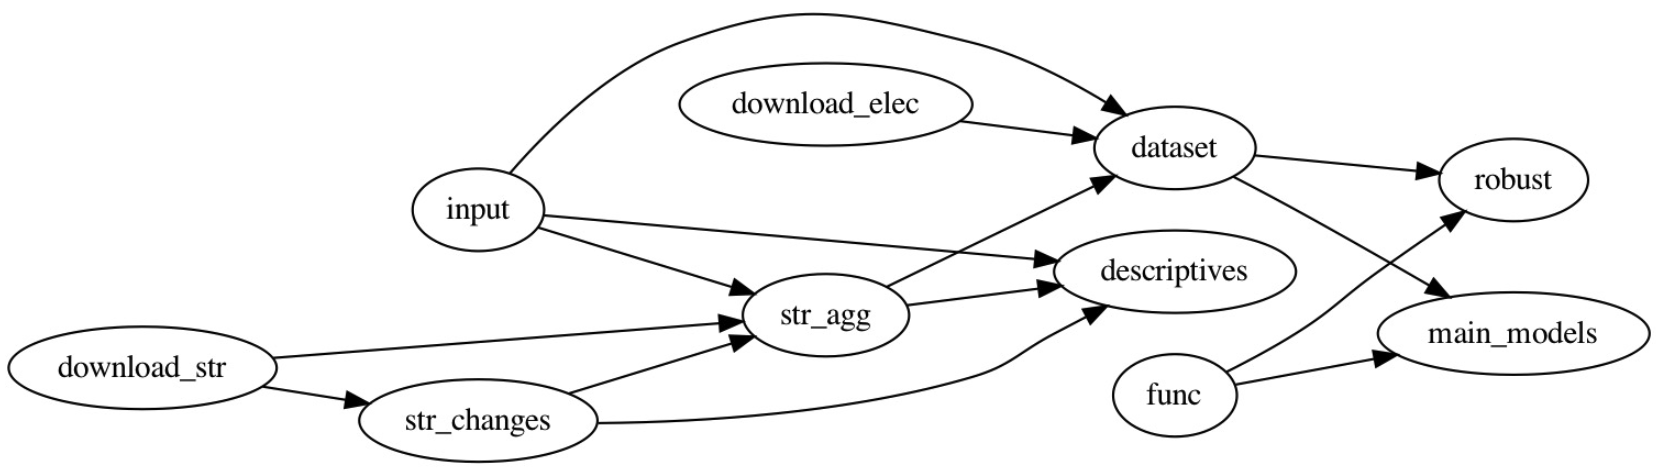
\includegraphics[width = \textwidth]{img/workflow_vox_streets}

\end{frame}
% ----------------------------------------------------

% ----------------------------------------------------
\begin{frame}
\frametitle{Automate stuff}
\centering

\begin{itemize}[<+->]
  \item Main idea is: you don't want to work twice, and you want to minimize errors
  \item This is very general, but I'd would say applies to three main things:
  \item[1.] A programming style, especially in \texttt{R}:
  \begin{itemize}
    \item Use functions whenever you can, save them in one file
    \item Do not write `constants' twice, and try to put them at the beginning
  \end{itemize}
  \item[2.] \textit{Code} the whole computing pipeline of a project, from data downloading or cleaning to producing the final PDF
  \begin{itemize}
    \item We'll see a nice tool for this: \textit{Makefile}
  \end{itemize}
  \item[3.] Use your computer to do things for you
  \begin{itemize}
    \item from joining all PDFs in a folder to updating/copying files to \href{https://github.com/franvillamil/franvillamil.github.io/blob/master/post_setting_up_macos.md}{configuring a new computer} to \href{https://github.com/franvillamil/franvillamil.github.io/blob/master/post_R_google_cloud.md}{setting up a virtual machine} to ...
    \item \texttt{baserepos} example
  \end{itemize}
\end{itemize}

\end{frame}
% ----------------------------------------------------

% ----------------------------------------------------
\begin{frame}
\frametitle{Automate data output and writing}
\centering

\begin{itemize}[<+->]
  \item When you translate R output to a writing form, an option would be:
  \begin{itemize}
    \item Produce plots in R, save them in files, add them to the Word file
    \item Create tables in R, copy them to a Word file (or better, create Latex code and copy \& paster it)
  \end{itemize}
  \item A better approach is to automate this:
  \begin{itemize}
    \item Automatically save all plots in a given folder directly from the R code, and do the same with the tables in plain text \texttt{.tex} files
    \item Call them from the \texttt{Latex} file directly from their original folders
  \end{itemize}
\end{itemize}

\end{frame}
% ----------------------------------------------------

% ----------------------------------------------------
\begin{frame}
\frametitle{Version control}
\centering

\begin{itemize}[<+->]
  \item \texttt{final1.docx}, \texttt{finalfinal.docx}... but in a proper way
  \item You want to keep control of all versions of a file, something like MS Word's `Tracked changes' but just much better
  \begin{itemize}
    \item Keep a time machine of all versions of a file
    \item Allow collaboration between different people (or between two computers)
  \end{itemize}
  \item There is more than one system, but we'll see \texttt{Git} (and Github)
\end{itemize}

\end{frame}
% ----------------------------------------------------

% ----------------------------------------------------
\begin{frame}
\frametitle{Version control}
\centering

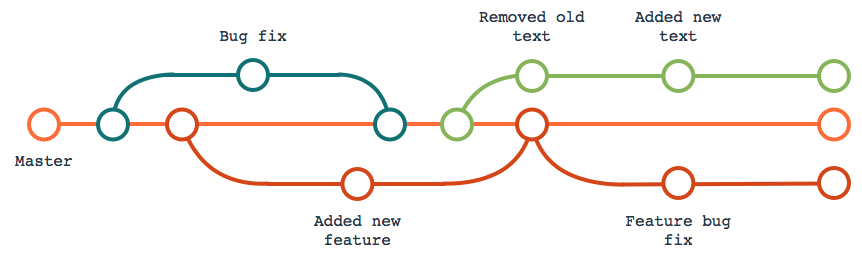
\includegraphics[width = \textwidth]{img/gitesquema}

\end{frame}
% ----------------------------------------------------

% ----------------------------------------------------
\begin{frame}
\frametitle{Version control}
\centering

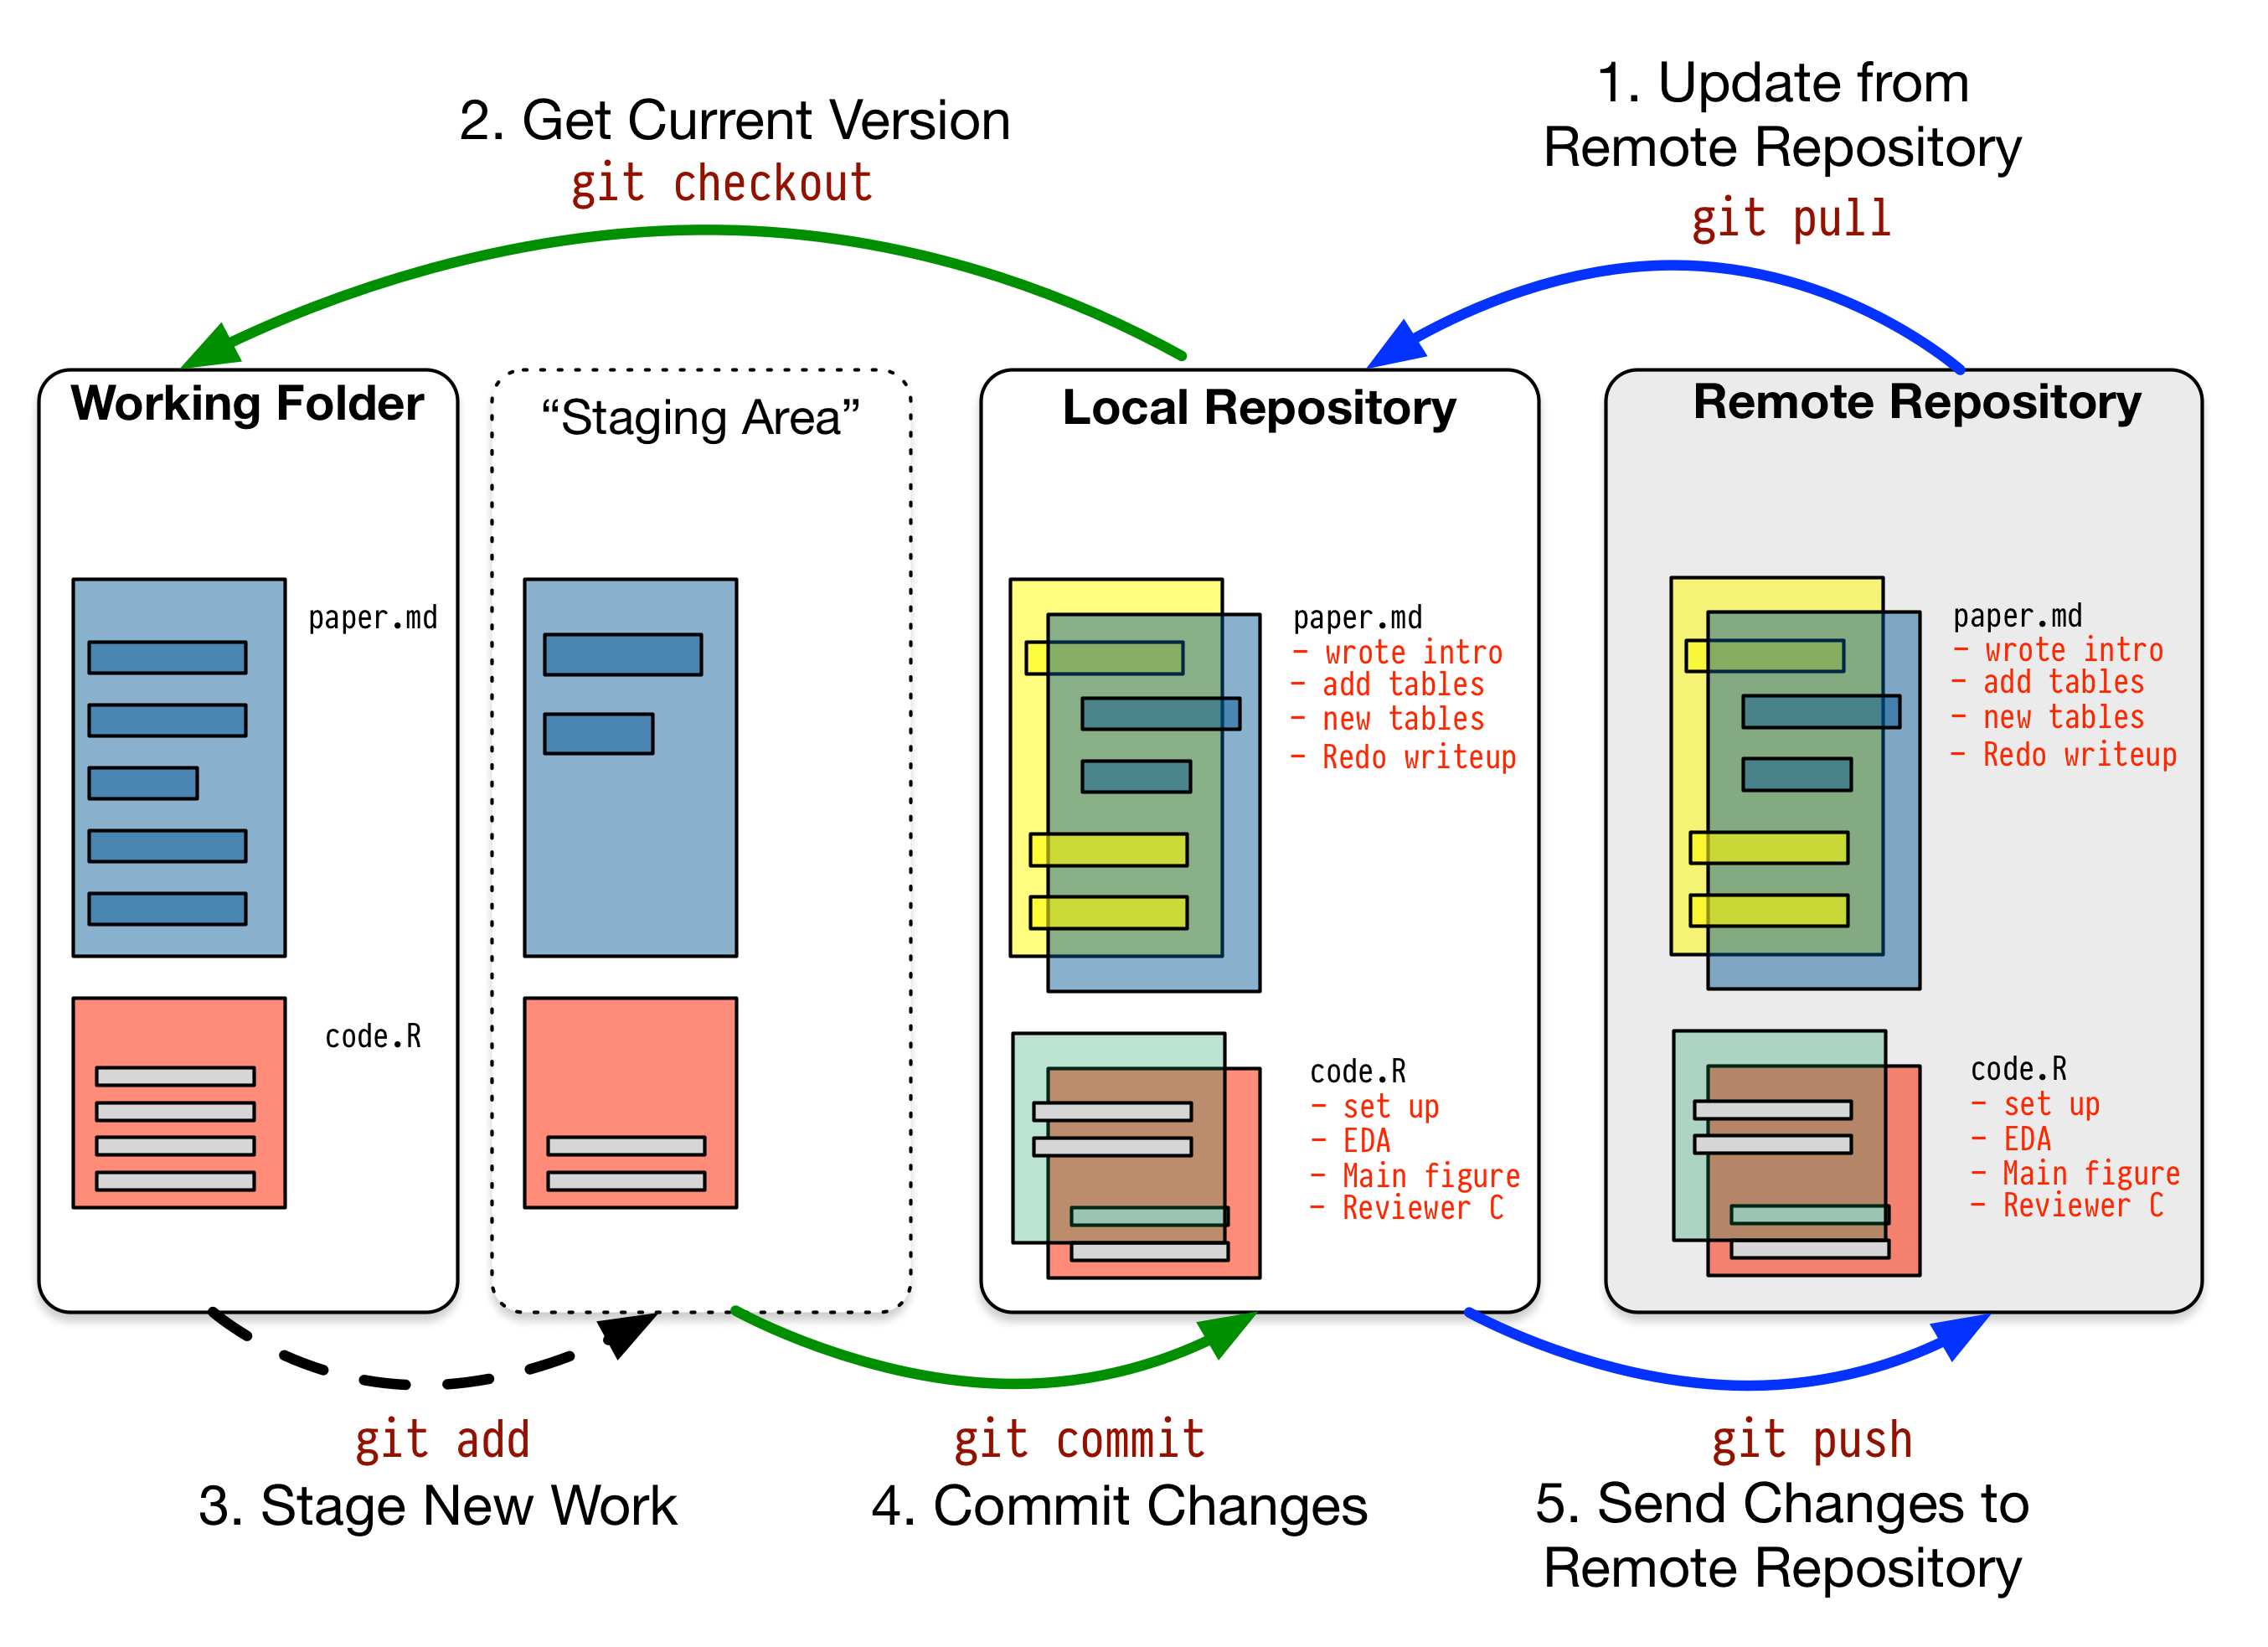
\includegraphics[width = \textwidth]{img/git-basic}

\end{frame}
% ----------------------------------------------------

% ----------------------------------------------------
\begin{frame}
\frametitle{Version control - a note}
\centering

\begin{itemize}
  \item Version control works \textbf{much} better if you work with other people who also use version control, which is often not the case (at least not mine)
  \item Yet, there are two advantages to use it in my view:
  \begin{itemize}
    \item Obvious one: keep older versions of a file
    \item If you work with two computers, perhaps Google Drive/Dropbox do not work that well
    \item Virtual machines (e.g. Google Cloud Computing, Amazon Web Services)
  \end{itemize}
\end{itemize}

\end{frame}
% ----------------------------------------------------

% ----------------------------------------------------
\begin{frame}
\frametitle{Basics of my workflow}
\centering

\begin{itemize}
  \item[1.] Keep one folder for each project, and within it, in each task goes in a separate folder, that contains: R (or \texttt{tex}) file, and an output folder
  \begin{itemize}
    \item You often need to save some initial files, I use a folder called `input`
  \end{itemize}
  \item[2.] \textbf{All} output from R is created automatically, \textbf{no manual changes}
  \begin{itemize}
    \item Save plots in PDF and use \href{https://vincentarelbundock.github.io/modelsummary/articles/modelsummary.html}{modelsummary}
  \end{itemize}
  \item[3.] Create a `writing' folder with the Latex files, from where you can access the analyses output
  \begin{itemize}
    \item Note to Overleaf users -- easier approach: a different project file, and a shell file to copy all output
    \item I use Github to save \texttt{.bib} files
  \end{itemize}
  \item[4.] Use version control, also to sync across computers
  \item[5.] (Less important) \textit{Makefile}

\end{itemize}

\end{frame}
% ----------------------------------------------------

% ----------------------------------------------------
\begin{frame}
\frametitle{A real example}
\centering

\begin{itemize}
  \item \href{https://github.com/franvillamil/streets_vox/}{https://github.com/franvillamil/streets\_vox/}
\end{itemize}

\end{frame}
% ----------------------------------------------------

% ----------------------------------------------------
\begin{frame}
\frametitle{Some resources}
\centering

\begin{itemize}
  \item Hadley Wickham's \href{http://adv-r.had.co.nz/Style.html}{R Style guide} (and the whole \href{http://adv-r.had.co.nz/}{Advanced R book} later on)
  \item Software Carpentry's lessons: \href{https://software-carpentry.org/lessons/}{https://software-carpentry.org/lessons/}
  \begin{itemize}
    \item Especially \href{https://swcarpentry.github.io/shell-novice/}{Unix Shell} and \href{https://swcarpentry.github.io/git-novice/}{Version Control with Git}
  \end{itemize}
  \item Kieran Healy's \textit{The Plain Person’s Guide to Plain Text Social Science}: \href{https://plain-text.co/}{https://plain-text.co/}
  \begin{itemize}
    \item Although \texttt{emacs} is perhaps a bit too hardcore
  \end{itemize}
  \item The best Git course I know is this: \href{https://gitexercises.fracz.com/}{https://gitexercises.fracz.com/}
  \item MIT's \textit{The Missing Semester of Your CS Education}: \href{https://missing.csail.mit.edu/}{https://missing.csail.mit.edu/}
\end{itemize}

\end{frame}
% ----------------------------------------------------

\end{document}
